\documentclass{article}
\usepackage[utf8]{inputenc}
\usepackage{graphicx}

\title{Relazione BJT}
\author{Francesco Pio Merafina, Onofrio Davide Caputo, Alessandro Lamesta}


\begin{document}

\maketitle

\section{Abstract:}
Lo scopo dell'esperimento è osservare l'effettivo effetto di amplificazione di un segnale in corrente alternata dovuta ad un transistor BJT in confiurazione ad emitter comune.
~
\section{Cenni Teorici:}
Il transistor BJT è ottenuto mediante l'unione di 3 cristalli di silicio drogati in modo diverso; i due esterni pesantemente e quello centrale in maniera leggera ed in modo diverso rispetto ai due esterni. Questo schema permette di avere amplificazione di correnti e tensioni alternate, sfruttando le barriere di potenziale presenti tra le due giunzioni e le correnti di diffusione tra le regioni a drogaggio diverso. Nel nostro esperimento abbiamo usato un transitor npn, cioè le regioni esterne drogate n e quella interna p. Lo schema da noi studiato è quello di un transistor BJT in configurazione ad emitter comune, cioè stimolazione sulla base (da ora in poi indicata come B), emitter (da ora in poi indicato con E) collegato a terra mediante una resistenza, e prelievo dell'output dal collettore (da ora in poi indicato con C). Prima di procedere alla misura il circuito è stato analizzato teoricamente, prima facendo una analisi in corrente continua e poi in corrente alternata, sfruttando dei modelli di schematizzazione del transistor noti dalla teoria.
Si è potuto fare ciò poichè ipotiziamo che il circuito ha un comportamento lineare e quindi vale il principio di sovrapposizione.
~
\begin{figure}[h!]
    \centering
    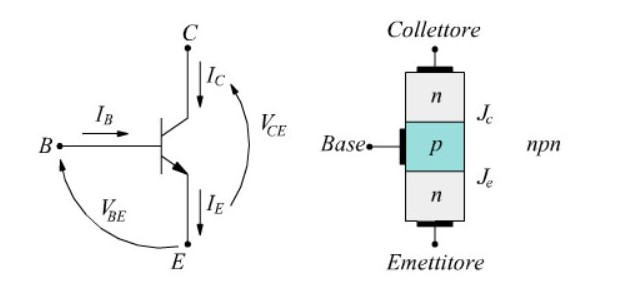
\includegraphics[width=\linewidth]{bjt.jpg}
    \caption{Simbolo circuitale a sinistra ed effettiva composizione di un transistor BJT npn a destra}
    \label{figura1}
\end{figure}
~
\begin{figure}[h!]
    \centering
    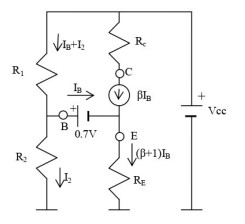
\includegraphics[width=\linewidth]{analisi dc bjt.jpg}
    \caption{Esempio di amplificatore BJT in configurazione emitter comune, analisi DC}
    \label{figura1}
\end{figure}
~
\begin{figure}[h!]
    \centering
    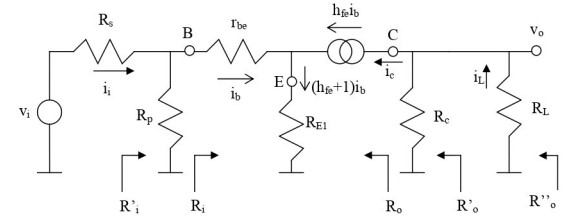
\includegraphics[width=\linewidth]{analisi ac bjt.jpg} 
    \caption{Esempio di amplificatore BJT in configurazione emitter comune, analisi AC}
    \label{figura1}
\end{figure}
~
\section{Strumentazione:}
La strumentazione utilizzata per l'esperienza consiste in:
\begin{itemize}
    \item -Transistor BJT  2N2222A
    \item -i seuenti resistori con tollerana del 5$\%$:1 resistore da 100$\Omega$, 2 resistori da 1k$\Omega$, 2 resitori da 10k$\Omega$, 1 resistore da 18k$\Omega$
    \item -3 capacitatori da 100 $\mu$F
    \item -Potenziometro da 10K$\Omega$
    \item -Potenziometro da 2.2K$\Omega$
    \item -Multimetro digitale usato come voltmetro
    \item -Amperometro analoigico
    \item -Generatore di tensione continua
    \item -Genereatore di tensione alternata
    \item -oscilloscopio
\end{itemize}
il tutto è stato montato su una scheda millefori usando dello stagno ed un saldatore.
~
\section{Metodologia di misura e risultati sperimentali:}
Come già detto prima di procedere alla misura effettiva si è fatta una analisi teorica per comprendere quali devono essere i parametri di tensioni e correnti dell'amplificatore, poiché da questi parametri possiamo determinare il punto di lavoro e quindi il gaudagno. Un parametro fondamentale del transistor è il coefficente $\beta$ il quale rappresenta il rapporto tra I$_{E}$ su I$_{B}$, e quindi possiamo teoricamente prevedere il guadagno, esso si può misurare dal tester digitale con una apposita funzione. Qui sotto è riportata una tabella con i valori teorici e quelli ricavati sperimentalmente dalla misura del circuito dei parametri in DC che determinano l'amplificazione in AC:
\begin{table}[]
    \begin{center}
        \begin{tabular}{c|c|c|}
         &Teorico&Sperimentale\\
      I$_{B}$&22.00$\mu$A&21.00$\pm$0.05$\mu$A\\
      I$_{C}$&4.20mA&4.16$\pm$0.05mA\\
      I$_{E}$&4.20mA&4.15$\pm$0.05mA\\
      V$_{CE}$&6.50V&6.47$\pm$0.5V\\
      $\beta$&200&197$\pm$5\\
      \end{tabular}
   \end{center}
\end{table} 
Quanto detto sopra riguarda l'analisi in DC, adesso passiamo alla trattazione AC. Per la misura si sono usate due sonde una collegata all'entrata ed una collegata al condensatore di disaccoppiamento del collettore, e mediante l'oscilloscopio valutiamo l'ampiezza dei due segnali, facendo variare la frequenza del segnale di input in modo da trovare la frequenza di taglio inferiore, la media banda dove il guadano è indipendente dalla frequenza, e la frequenza di taglio superiore, di seguito i risultati ed il grafico:
\begin{table}[]
    \begin{center}
        \begin{tabular}{|c|c|c|}
        Frequenza [Hz]&Guadagno&u$_{G}$\\
      10&4.20&0.20\\
      30&7.06&0.25\\
      100&8.10&0.20\\
      300&8.50&0.31\\
      1K&8.35&0.30\\
      3K&8.45&0.28\\
      10K&8.35&0.30\\
      30K&8.50&0.27\\
      100K&8.40&0.31\\
      300K&8.47&0.29\\
      1M&8.30&0.30\\
      3M&7.90&0.25\\
      10M&5.00&0.20
      \end{tabular}
   \end{center}
\end{table} 
~
\begin{figure}[h!]
    \centering
    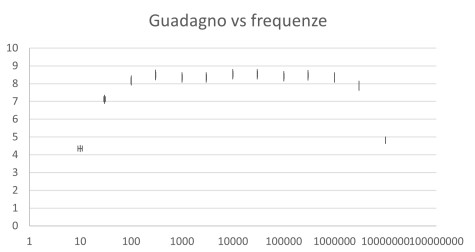
\includegraphics[width=\linewidth]{guadagno bjt.jpg}
    \caption{grafico del guadagno al variare della frequenza}
    \label{figura1}
\end{figure}
~
inoltre sappiamo che il guadagno dellamplificatore è:
\begin{equation}
    A_{v}=-\frac{\beta R_{0}}{R_{i}}
\end{equation}
Quindi siamo interessati nel valutare sperimentalmente il valore delle due resistenze di input ed output del segnale, le quali sono state valutate teoricamente analizando il circuito il AC. Per misurarle è stato utilizato il metodo del dimezzamento, cioè abbiamo inserito un potenziometro in serie all'input ed all'output e valutiamo il rapporto delle due tensioni prima e dopo il potenziometro, per comodità si porta il segnale alla metà del valore senza potenziometro così da poter ottenere subito il valore della resistenza valutandola usando il tester come ohmetro, per la scelta del potenziometro si usa come riferimento dell'ordine di grandezza il valore teorico, si è ottenuto:
\begin{table}[]
    \begin{center}
        \begin{tabular}{c|c|c}
         &Teorico&Sperimentale\\
      R$_{i}$&4.80K$\Omega$&4.79$\pm$0.50K$\Omega$\\
      R$_{o}$&0.90K$\Omega$&0.93$\pm$0.05K$\Omega$\\
         \end{tabular}
   \end{center}
\end{table} 
~
\section{Conclusioni:}
In conclusione possiamo affermare che effettivamente il BJT ha un comportamento di amplificazione della tensione previsto dalla configurazione ad emitter comune, e che i modelli da noi utilizati per sviluppare il l'analisi del circuito funzionano perfettamente
~
\section{Appendice:}
Testi di riferimento:
\begin{itemize}
    \item Sedra, Smith, Microelectronic circuits, 5th ed. Oxford University Press,
2004
    \item Dell’Orso, Falchini, Flaminio et al. Introduzione all’elettronica digitale,
parte 2, Edizioni ETS, 2005

\end{itemize}

\end{document}
